%-------------------------------------------------------------------------------
% playlist
%-------------------------------------------------------------------------------
%
% \file        playlist.tex
% \library     Documents
% \author      Chris Ahlstrom
% \date        2018-09-15
% \update      2021-06-13
% \version     $Revision$
% \license     $XPC_GPL_LICENSE$
%
%     Provides a discussion of the playlist functions that Seq66 supports.
%
%-------------------------------------------------------------------------------

\section{Seq66 Play-Lists}
\label{sec:playlist}

   \textsl{Seq66} supports play-lists.
   A play-list is a variation on the 'rc' file, conventionally ending with the
   extension \texttt{.playlist}.  It contains a number of "playlist" sections,
   each with a human-readable title, selectable via a MIDI data number,
   or by moving to the next or previous playlist in the list using the
   \texttt{Up} and \texttt{Down} arrow keys.
   Each playlist section contains a list of songs, also selectable via a MIDI
   data number, or by moving to the next or previous song in the list using the
   \texttt{Left} and \texttt{Right} arrow keys.

   Movement between the playlists and the songs is accomplished via 
   MIDI control or the arrow keys.
   it describes the general usage of the [midi-control] section.
   Using MIDI control makes it possible to use the \texttt{seq66cli}
   headless version of \textsl{Seq66} in a live setting.
   In the normal user-interface, play-list movement
   can also be done manually via the four arrow keys on the computer
   keyboard.

   The playlist file can be specified on the command-line, in
   the 'rc' file, or be loaded
   from the \textbf{File / Open Playlist} menu.
   If it is specified on the command line, that playlist setup will
   be written to the 'rc' file.  It can be removed by specifying a blank (i.e.
   two double-quotes, "") play-list name.
   The file extension is \texttt{.playlist}.

   The Qt user-interface supports editing of the play-list, though not yet
   perfected; bugs still exist.
   The user can use a text editor to edit the play-list file, if careful.

   The play-list format is defined in the following section.
   Later sections describe the user-interface.

\subsection{Seq66 Play-Lists / 'playlist' File Format}
\label{subsec:playlist_setup}

   The play-list file, by convention, has a file-name of the form
   \texttt{sample.playlist}.
   The play-list file starts with a hardwired top banner that the user can edit
   with a text editor.  It can also have an optional comments section, much
   like the 'rc' and 'usr' files.  It is \textsl{not} overwritten
   when \textsl{Seq66} exits.

   \begin{verbatim}
   [comments]
   Comments added to this section are preserved....
   \end{verbatim}

   A blank line (without even a space) ends the comment section.
   Following the comments section is a \texttt{[playlist-options]} section.

   \begin{verbatim}
   [playlist-options]
   unmute-new-song = true   # a new song selection unmutes its patterns
   deep-verify = false      # If true, every MIDI song is opened and verified
   \end{verbatim}

   The first option allows the load of the next song to enable the patterns in
   that song.
   The second option causes each MIDI file to be opened to verify that it is an
   error-free play-list.  This process can be time-consuming for large
   playlists.  If set to false, \textsl{Seq66} still makes sure each MIDI
   file exists.

   Following the options section are one or more \texttt{[playlist]} sections.
   Here is the layout of a sample playlist section.

   \begin{verbatim}
   [playlist]

   # Playlist number, arbitrary but unique. 0 to 127 recommended for MIDI control

   number = 126
   name = "Music for Serious Dogs"  # Display name of this play list
   directory = "contrib/midi/"      # Storage directory for the tunes

   # Provides the song-control number and the base file-name of each song in
   # this playlist.  The playlist directory is used, unless the
   # file-name contains a path.

   70 "allofarow.mid"
   71 "CountryStrum.midi"
   72 "contrib/wrk/longhair.wrk"
   \end{verbatim}

   \index{playlist!tag}
   A play-list file can have more than one \texttt{[playlist]} section.  This
   allows for partitioning songs into various groups that can be easily
   selected (e.g. based on the mood of the musician or the audience).

   \index{playlist!number}
   After the \texttt{[playlist]} tag comes the play-list number.
   This number can be any non-negative value.
   However, in order to use MIDI control to select the playlist, this number
   should be limited to the range 0 to 127.
   If there is more than one \texttt{[playlist]} section, they are ordered by
   this number, regardless of where they sit in the play-list file.

   \index{playlist!title}
   Next comes a human-readable name for the playlist, which is meant to be
   displayed in the user-interface.  If surrounded by quotes, the quotes are
   removed before usage.

   \index{playlist!song-storage directory}
   Next is the song-storage directory.
   This directory is the default location in which to find the songs.
   It can be an absolute directory or a relative directory.
   However, be wary of using relative directories, since they depend on where
   \textsl{Seq66} is run.
   Also, if a song's file-name  has its own directory component, that overrides
   the default song-storage directory.

   Lastly, there is a list of MIDI song file-names, preceded by their numbers.
   As with the playlist numbers, it is recommended to keep them between 0 and
   127, for usage with MIDI control.  And the songs are ordered by this number,
   rather than by their position in the list.

\subsection{Seq66 Play-Lists / 'rc' File}
\label{subsec:playlist_rc_file}

   The most consistent way to specify a play-list is to add an entry like the
   following to the 'rc' file:

   \begin{verbatim}
   [playlist]
   # Provides a configured play-list and a flag to activate it.
   0     # playlist_active, 1 = active, 0 = do not use it
   # Provides the name of a play-list.  If there is none, use '""'.
   # Or set the flag above to 0.
   "/home/ahlstrom/.config/seq66/sample.playlist"
   \end{verbatim}

   This setup allows a play-list file to be specified and activated.
   If the name of the play-list file does \textsl{not} contain a directory,
   then the play-list file is search for in the user's \textsl{Seq66}
   configuration directory.

   If the play-list file-name is empty (i.e. set to \texttt{""}, then there is
   no play-list active.

\subsection{Seq66 Play-Lists / 'ctrl' File / [midi-control]}
\label{subsec:playlist_rc_file_midi_ctrl}

   The MIDI control stanzas for play-list and song-selection don't quite follow
   the toggle/on/off convention of the \texttt{[midi-control]} section, though
   the layout is the same:

   \begin{verbatim}
                Pick-by-number     Next            Previous
      24 "F2" [ 144 2 1 127 ] [ 144 4 1 127 ] [ 144 0 1 127 ] # Play List
      25 "F3" [ 144 5 1 127 ] [ 144 3 1 127 ] [ 144 1 1 127 ] # Play Song
   \end{verbatim}

   Both lines specify setting the next playlist or song according to a number,
   or via "next" and "previous" controls.  The "next" and "previous" controls
   can be implemented by any MIDI event, including \textsl{Note On} or
   \textsl{Program Change}.  However, the "value" section requires a MIDI event
   that provides a \texttt{d1} (second data byte) value, because this value is
   used as the MIDI control number to select a playlist or song item.
   So, the following setting,

   \begin{verbatim}
      24 "F2" [ 0x90  2  1 127] . . .
   \end{verbatim}

   specifies that a \textsl{Note On} event with channel 0 (144 = 0x90) on note
   \#2 with a velocity between the range 1 to 127 will select a play-list.
   However, this selection will be made only if the velocity ranges from 1 to
   127, and there exists a selection with that velocity in the play-list file.
   This control requires a controller device that can be configured to provide
   the exact \textsl{Note On} event, including the exact velocity.

\subsection{Seq66 Play-Lists / Command Line Invocation}
\label{subsec:playlist_cmd_line}

   The command-line options to specify (and activate) the play-list feature
   are:

   \begin{verbatim}
      -X playlist_file
      --playlist playlist_file
   \end{verbatim}

   The play-list file is either a base-name (e.g. \texttt{sample.playlist})
   or a name that includes the full path to the play-list file
   (e.g. \texttt{data/sample.playlist}).
   If no path is specified, the directory is the currently set
   \textsl{Seq66} configuration-file directory.
   For session support, one must stick with the configuration directory;
   do not provide an explicit directory-name.

   Please note that any play-list file specified on the command line, or loaded
   in the play-list user-interface,
   will be written into the 'rc' file's \texttt{[playlist]} section when
   \textsl{Seq66} exits.

\subsection{Seq66 Play-Lists / Verification}
\label{subsec:playlist_verify}

   When \textsl{Seq66} loads a play-list file, an option allows every
   song in the play-list file to be verified by loading it.  If any load fails,
   then the playlist will fail to load.  This check can be slow when there are
   many large MIDI files specified in the play-list file.

\subsection{Seq66 Play-Lists / User Interface}
\label{subsec:playlist_uis}

   Playlists and songs can be selected or moved-to via keystrokes or
   user-interface actions, in addition to MIDI control.

   The \texttt{Up} and \texttt{Down} arrows move forward or backward through
   the list of play-lists, and the
   The \texttt{Right} and \texttt{Left} arrows move forward or backward through
   the list of songs for the currently-selected play-list.

   The Qt 5 user-interface supports the display, selection, and editing of
   the play-lists and the song-list for each play-list.
   There are still some minor issues to work out.  If encountered, close
   \textsl{Seq66} and edit the \texttt{.playlist} file manually.
   It is self-documenting.

\begin{figure}[H]
   \centering 
   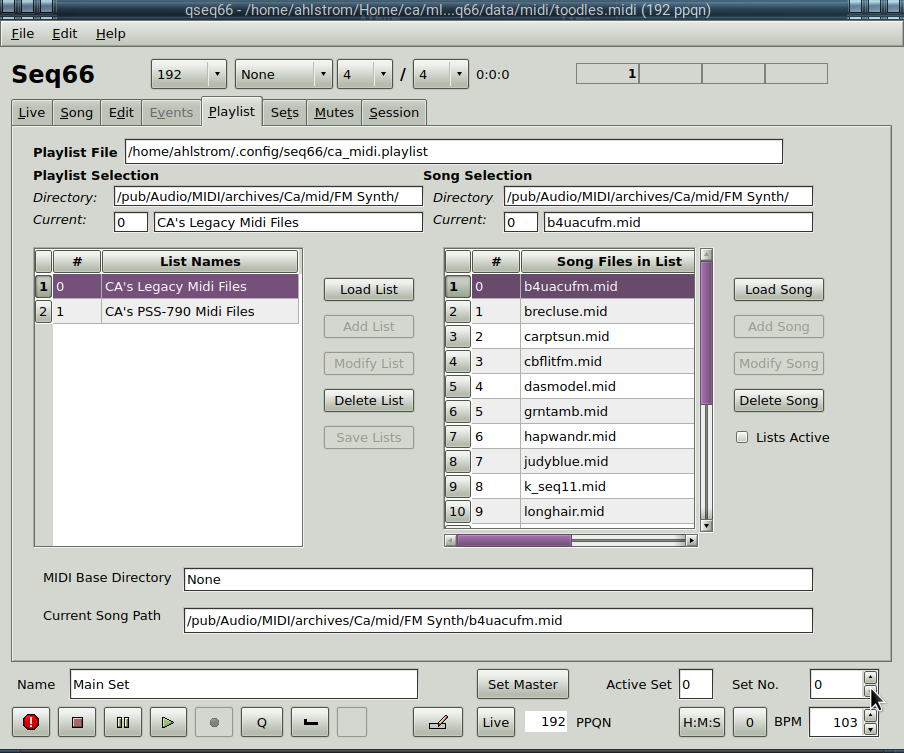
\includegraphics[scale=0.65]{tabs/playlist/personal-playlist-light.png}
   \caption*{Qt 5 Playlist Tab}
\end{figure}

   There is a lot to talk about in this tab.

   \begin{enumber}
      \item \textbf{Playlist File}.
         This field displays the path to the loaded
         play-list file.  It is not editable.  Remember that
         a play-list file can contain multiple play-lists.
      \item \textbf{Playlist Selection}.
         These fields display the main MIDI-file directory,
         the MIDI control number, and the name of the selected play-list.
         The \textbf{Directory} is where the MIDI files reside by default.
         A file-name can include a different path, however.
         These fields are editable, with the intent to use them to add a new
         play-list or modify the current one.
      \item \textbf{Song Selection}.
         These fields display the MIDI-file directory,
         the MIDI control number, and the file-name of the selected play-list.
         Note that the directory is normally the play-list directory, but a
         path present in the MIDI file-name overrides that directory, and then
         an asterisk is shown to flag that status.
         Only the MIDI control number field is editable,
         with the intent to use it to add a new
         song.
      \item \textbf{List Names}.
         This table shows the MIDI-control number and
         the name of each play-list.
      \item \textbf{List Buttons}.
         These buttons are described below.
         Please note that, in some cases, the exact functionality is still
         being worked out or perfected.
      \item \textbf{Song Files in List}.
         This table shows the MIDI-control number and
         the name of each song.
      \item \textbf{Song Files in List Buttons}.
         These buttons are described below.
         Please note that, in some cases, the exact functionality is still
         being worked out or perfected.
   \end{enumber}

\subsubsection{Seq66 Play-Lists / User Interfaces / Playlist Buttons}
\label{subsubsec:playlist_ui_playlist_buttons}

   This section briefly describes the "List" buttons to the right of the
   play-list table.

   \begin{itemize}
      \item \textbf{Load List}.
      \item \textbf{Add List}.
      \item \textbf{Modify List}.
      \item \textbf{Delete List}.
      \item \textbf{Save Lists}.
   \end{itemize}

   \setcounter{ItemCounter}{0}      % Reset the ItemCounter for this list.

   \itempar{Load List}{playlist editor!load list}
   This button brings up the "Open play-list file" dialog, using the
   \textsl{Seq66} configuration directory as the default directory.
   It is recommended to use only this directory, especially when running in a
   session manager. If loaded from somewhere else, save the file back to the
   configuration directory.

   \itempar{Add List}{playlist editor!add list}
   This button is enabled with the editing of the \textbf{Playlist Selection}
   fields.  Once these three fields are correct, the list can be added.
   The new list can then be populated with songs.

   \itempar{Modify List}{playlist editor!add list}
   This button is enabled with the editing of the \textbf{Playlist Selection}
   fields.  Once these three fields are correct, the list can be modified.
   \textbf{Bug: Currently does not work.}

   \itempar{Delete List}{playlist editor!delete list}
   This button removes the currently-selected play-list from the play-list
   file.  This action doesn't take effect until the play-list file is saved or
   \textsl{Seq66} exits and does its normal saving.

   \itempar{Save Lists}{playlist editor!save lists}
   This button bring up a file dialog to save the current play-lists and songs
   into a play-list file.

   This section briefly describes the "Song" buttons to the right of the
   song-list table.

   \begin{itemize}
      \item \textbf{Load Song}.
      \item \textbf{Add Song}.
      \item \textbf{Modify Song}.
      \item \textbf{Delete Song}.
      \item \textbf{Lists Active}.
   \end{itemize}

   \setcounter{ItemCounter}{0}      % Reset the ItemCounter for this list.

   \itempar{Load Song}{playlist editor!load song}
   This button bring up a dialog to open a MIDI or WRK file from
   the current song-directory or from an arbitrary directory.
   Currently, be careful with this option; adding a file from an arbitrary
   directory will generally prepend that directory to the MIDI file-name,
   making the song list difficult to read.

   \itempar{Add Song}{playlist editor!add song}
   This button is meant to add a song already loaded in the \textbf{Live} frame
   into the play-list.  Just open a new tune, test it, and then add it to the
   play list.  Note that currently one may load a new tune into the playlist
   from anywhere a song is allowed to be loaded by the session.

   \itempar{Modify Song}{playlist editor!modify song}
   This button is meant to modify song information.  However, the only item
   that can be altered is the MIDI control number.

   \itempar{Delete Song}{playlist editor!delete song}
   This button deletes the currently-selected song from the song list.

   \itempar{Lists Active}{playlist editor!lists active}
   If checked, the play-list is enabled, and the arrow keys, automation keys,
   and MIDI controls (if configured) can be used to move between play-lists and
   songs.

\subsubsection{Seq66 Play-Lists / User Interfaces / Info Fields}
\label{subsubsec:playlist_ui_info_fields}

   The following read-only fields show some information about the file-system
   for the play-lists.

   \begin{itemize}
      \item \textbf{MIDI Base Directory}.
         Provides the top-most directory where all of the files in the
         play-list are stored.
         Currently read-only, in order not to interfere with session locations.
      \item \textbf{Current Song Path}.
         Shows the exact path the the currently-selected song.
         Currently read-only, in order not to interfere with session locations.
   \end{itemize}

   These items can be modified, however, by editing the play-list file
   directly.

%-------------------------------------------------------------------------------
% vim: ts=3 sw=3 et ft=tex
%-------------------------------------------------------------------------------
